\documentclass[../main]{subfiles}

\graphicspath{{../figures/}}

\begin{document}

\chapter{提案手法}
\label{cp:proposed_method}
\thispagestyle{empty}
\minitoc
\newpage

\section{はじめに}
\label{sec:pmethod_introduction}

本章では，車椅子卓球選手の競技中の動作の測定と解析のアプローチについて述べる．

\refsec{sec:approach}では，本研究のアプローチについて述べる．

\refsec{sec:pmethod_model}では，本研究の実験概要について述べる．

\refsec{sec:analysis_method1}では，画像解析を用いた解析手法について述べる．

\refsec{sec:analysis_method2}では，筋活動による解析手法について具体的に述べる．

最後に\refsec{sec:pmethod_conclusion}では，本章のまとめを述べる．

\clearpage

\section{本研究のアプローチ}
\label{sec:approach}
本研究では、個人の身体機能差が著しい車椅子卓球選手において、打球の正確性を決定づける要因を解明することを目指す。従来のキネマティクス中心の解析や、単一時点の統計処理による一般化とは異なり、本研究では動作の駆動源である筋活動の時系列パターンに着目する。

図\ref{fig:exp_setup}に本研究で提案する解析プロセスの概要を示す。実際のラリー中における選手の身体動作（モーションキャプチャ）と筋活動（表面筋電図）、およびその結果としての打球の正確性を同期計測する。

具体的には、計測された筋活動の時系列データを入力とし、打球の着弾誤差を出力とする機械学習モデルを構築する。このモデルは、インパクトの瞬間だけでなく、スイング開始前の準備局面を含む時間的な依存関係を学習する。さらに、学習済みモデルに対して Permutation Feature Importance（PFI）を適用することで、打球の成否に寄与する重要な筋群とその活動タイミングを定量的に特定する。

以上より、本研究では単なる動作観察では捉えきれない、パフォーマンスに直結する筋活動の時系列的な特徴を抽出し、客観的かつ説明可能な評価を行う。

\begin{figure}[t]
  \centering
  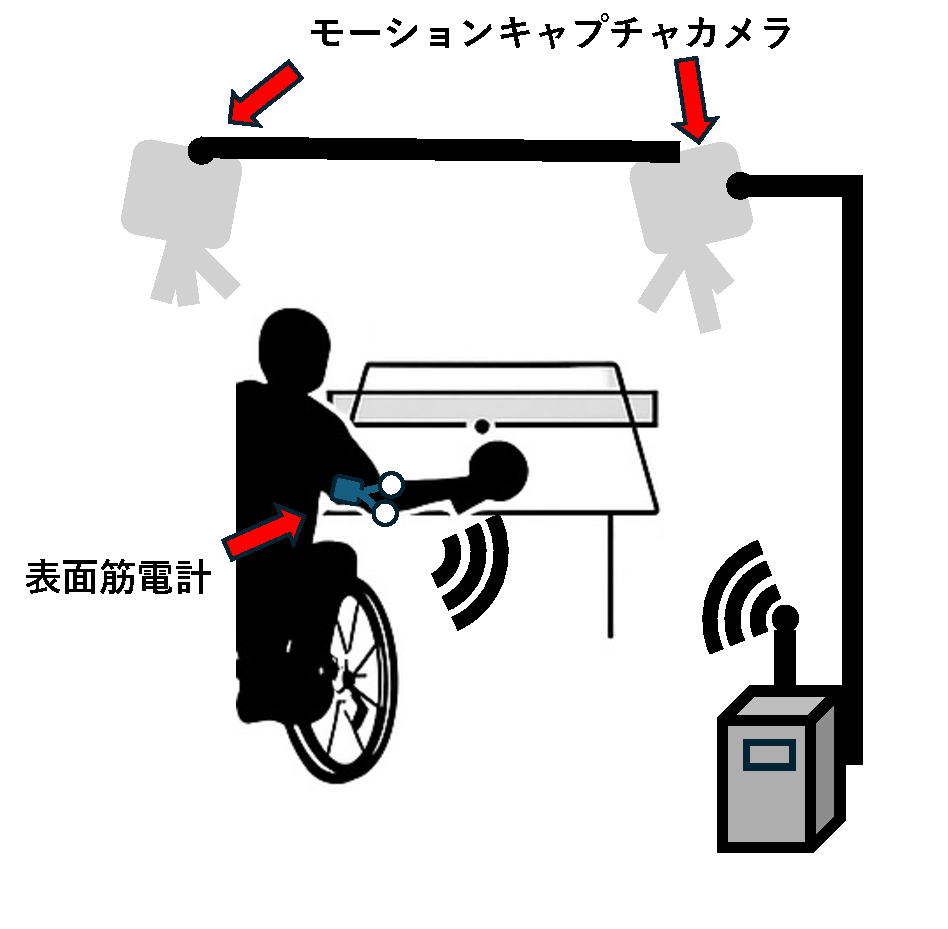
\includegraphics[keepaspectratio, width=0.8\linewidth]{chap2/exp_setup.pdf}
  \caption{計測システムの構成}
  \label{fig:exp_setup}
\end{figure}

\section{実験概要}
\label{sec:pmethod_model}
本節では，提案手法の構築および検証のために実施した計測実験の詳細について述べる．
本実験では，車椅子卓球選手の実際のラリー動作を対象に，身体動作，筋活動，およびボールの軌道情報を同期計測した．
以下，\ref{subsec:exp_person}項では実験参加者の属性について，\ref{subsec:exp_env}項では使用した計測機器と環境について，\ref{subsec:exp_method}項では具体的な実験課題と手順についてそれぞれ記述する．

\subsection{実験参加者}
\label{subsec:exp_person}
本研究の実験参加者は，パラリンピック車椅子卓球競技クラス4に所属する男子選手1名（年齢：26歳，利き手：右）とした．

被験者は，二分脊椎に起因する第3腰髄（L3）レベルの機能障害を有している．この障害レベルでは，座位バランスはある程度保持されるものの，下肢による強固な身体固定や重心移動が制限されるため，競技動作において上肢および体幹の協調的な制御が不可欠となる．

なお，実験に先立ち，被験者および実験協力者（コーチ）に対して本研究の目的，実験手順，および身体への負担や安全性について十分に説明を行い，書面による同意を得た．本研究は，東京大学倫理審査委員会の承認（承認番号：E2025ALS171）を得て実施された．

\subsection{計測環境}
\label{subsec:exp_env}
本実験における計測システムの構成を図\ref{fig:exp_setup}に示している．図の通り本実験は，表面筋電計，モーションキャプチャカメラを用いた同時計測システムを構築し，車椅子卓球選手のラリー中の運動データを収集，解析する．
身体動作およびボールの3次元位置計測には，光学式モーションキャプチャカメラ（Qualisys Miqus3, Qualisys社）20台を用いた．サンプリング周波数は300Hzとした．反射マーカーは，卓球台および被験者の車椅子，ラケットに貼付した．

禁活動の計測には，表面筋電計（Wave Infinity，Cometa社）を用いた．サンプリング周波数は2000Hzとした．フリーハンド側の筋活動がラリー中における車椅子操 作や体幹のバランス保持が打球精度に重要な役割を果 たしていると考えられるため，ラケットを保持するラケ ットハンド側に加えて両側を計測対象とした.
対象とした筋群は以下に示す通りである\ref{fig:muscle}：体幹部（大胸筋，腹直筋，腹斜筋，僧帽筋（上部，中部），広背筋，脊柱起立筋），上肢（三角筋（前部，後部），上腕二頭筋，上腕三頭筋，手根屈筋，手根伸筋，腕橈骨筋）など左右計28部位とした．

空間座標系は，右手系直交座標系を用いた．卓球台の中央を原点$(0, 0, 0)$とし，卓球台の長軸方向をX軸（選手視点でのネット方向を正），短軸方向をY軸（左側を正），鉛直上向をZ軸と定義した．

なお，動作計測システムと筋電計測システムは同期させてデータを取得し，時間的整合性を担保した．




\begin{figure}[t]
  \centering
  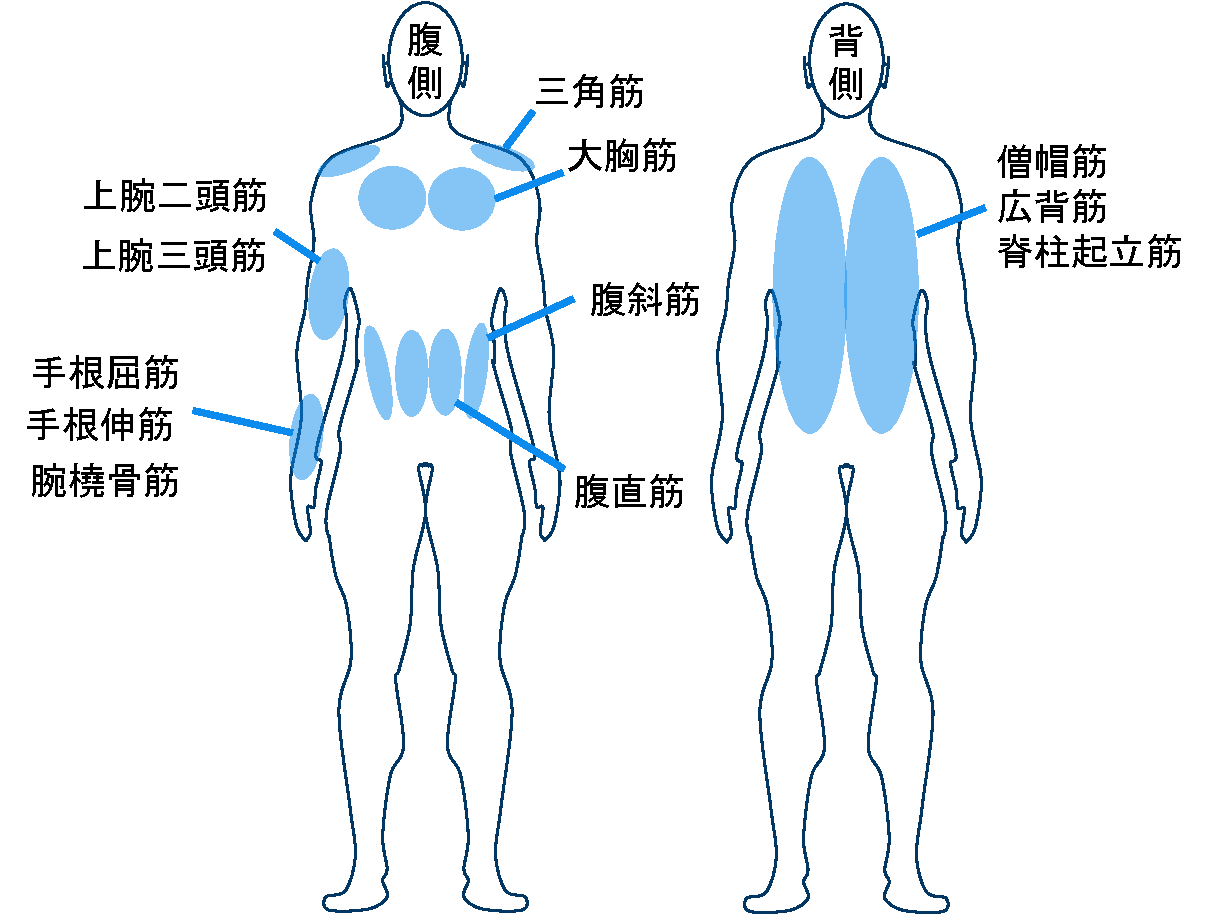
\includegraphics[keepaspectratio, width=1.0\linewidth]{chap2/muscle.pdf}
  \caption{対象とした筋群}
  \label{fig:muscle}
\end{figure}


\subsection{実験方法}
\label{subsec:exp_method}
実験課題は，コーチによる球出しに対するフォアハンドラリーとした．実際の試合場面における「揺さぶり」への対応能力を評価するため，コーチは，被験者の体に近い位置と体から遠い位置へ交互にボールを送球した．被験者には，送球されたボールを対角線上の卓球台の角（左端）に向けて，できるだけ速く，かつ正確に打ち返すよう指示した．
\clearpage

\section{画像解析を用いた解析手法}
\label{sec:analysis_method1}
本節では，録画された動画像データからボールの3次元挙動を復元し，打球の正確性を定量的に評価するとともに，その傾向を可視化する一連のプロセスについて述べる． 解析の全体フローは，1）手作業によるイベント区間の特定（アノテーション），2）ステレオ計測による3次元座標群の抽出，3）ターゲット到達精度の算出，4）精度の空間分布を可視化するショットマップの作成，の4段階から構成される．
ボールの空間位置を特定するため，2台の高速度カメラを用いたステレオ計測法を適用した．また解析には数値解析ソフトウェアMATLABを使用した．具体的な手順を本節では説明する．

\subsubsection{アノテーションと座標取得}
\label{subsec:annotation}
まず，各試行の録画データに対して手作業によるアノテーションを実施した．打球動作における重要局面であるラケットによるインパクトの瞬間（打点）および卓球台へのバウンドの瞬間（着弾点）に対応するフレーム番号を特定した．次に，特定された各フレームにおいて，左右のカメラ画像上のボール中心位置を目視にて特定し，その2次元画像座標 $(u, v)$ を記録した．これらの画像座標と，事前に実施したカメラキャリブレーションにより得られたカメラパラメータ（内部・外部パラメータ）を用いて，三角測量の原理に基づく3次元復元を行い，複数台のカメラによって撮影した画像から，対象空間におけるボールの3次元座標 $(x, y, z)$ を算出した．



\subsection{打球精度の定義と算出}
\label{subsec:shotaccuracy}
本研究における実験課題はクロス方向へのラリーであり，目標とする着弾点を卓球台の左端コーナー付近に設定した．
打球の正確性を評価するため，着弾点の3次元座標を卓球台平面（$xy$平面）に投影し，目標の座標との平面距離を算出した．

各試行 $i$ における着弾位置の水平座標を $(x_{land}^{(i)}, y_{land}^{(i)})$，目標とするターゲット位置の座標を $(x_{target}, y_{target})$ と定義する．
このとき，打球の誤差距離（Error Distance）$D_{err}^{(i)}$ は，以下の式に示す $xy$ 平面上でのユークリッド距離として定義される．

\begin{equation}
D_{err}^{(i)} = \sqrt{(x_{land}^{(i)} - x_{target})^2 + (y_{land}^{(i)} - y_{target})^2}
\end{equation}

ここで，$D_{err}^{(i)}$ が $0$ に近いほど，目標に対して正確に着弾したことを意味し，値が大きいほどターゲットから逸脱した打球であることを示す．
本解析では，この誤差距離 $D_{err}$ の値を，後述するショットマップの色付けおよび機械学習モデルの出力変数（回帰ターゲット）として使用した．

\subsection{ショットマップによる空間的傾向の可視化}
\label{subsec:shotmap}
算出された打球誤差と，打球位置の空間的な関係性を明らかにするため，詳細なショットマップを作成した．従来のショットマップは着弾位置をプロットするのが一般的であるが，本研究ではどの位置でボールを捉えた時に，高精度な打球が可能となるかという身体制御と結果の因果関係を検証するため，以下の手法を用いた．
\begin{enumerate}\item
  \textbf{プロット位置：} グラフ上の点の位置は，各試行におけるインパクト時のボール位置（打点）の3次元座標 $(x_{hit}, y_{hit}, z_{hit})$ に対応する．
  \item \textbf{カラーマッピング：} 各点の色情報は，前項で算出した着弾誤差距離 $D_{err}$ に基づいて決定される．
\end{enumerate}
具体的には，誤差距離 $D_{err}$ が小さい（精度が高い）試行を青色や緑色などの寒色系で，誤差が大きい（精度が低い）試行を赤色などの暖色系で表現し，その中間を連続的なカラーグラデーションで表示した．これにより，被験者が空間上のどの領域（例：身体の近く，あるいは高い打点など）でインパクトした際に，ターゲットに近い有効打を放つことができたかを直感的に把握することを可能とした．


\clearpage

\section{筋活動の解析手法}
\label{sec:analysis_method2}
本節では，計測された生体信号から，打球精度に影響を与える要因を抽出するための時系列解析手法について述べる．

\subsection{データの前処理}
\label{subsec:preprocess}
取得した表面筋電図（EMG）信号に対し，以下の信号処理を適用した． まず，生体信号に含まれるハムノイズおよび低周波のモーションアーチファクトを除去するため，40$\sim$400Hzのバンドパスフィルタを適用した ．次に，筋活動の振幅レベルを評価するために整流処理を行い，その後，平滑化処理を施して包絡線を算出した ． 最後に，機械学習モデルへの入力として各チャンネル間のスケールを統一するため，各試行のデータに対して正規化処理を行い ，これを解析用データとした．

\subsection{データセットの構築}
\label{subsec:dataset}
解析対象とする時間区間は，ボールインパクトの瞬間（$t=0$）を基準とし，スイング動作の開始前からインパクトまでの「準備局面」を含む区間とした．具体的には，インパクト前$1.0$秒から$0.0$秒までの時系列データを抽出した．
入力データ $X$ は，前処理を行った多チャンネルのEMG時系列で0田を採用した．出力データ $Y$ には，前節で算出した打球誤差 $E_i$ （目標からの距離）を教師ラベルを付与した．
これにより，筋活動パターンから打球の正確性を予測する回帰モデルの構築を行った．

\subsection{LSTMモデルによる要因解析}
打球動作のような一連の時系列データにおいては，ある瞬間の値だけでなく，時間的な変化のパターンが重要である．そこで本研究では，時系列データの学習に適し，長期的な依存関係を学習可能な再帰型ニューラルネットワーク（RNN）の一種である Long Short-Term Memory (LSTM) を採用した．

構築したモデルは，入力層，LSTM層，全結合層，出力層から構成される．本モデルを用いて打球精度の予測学習を行い，高い予測精度が得られることを確認した上で，モデルの解釈性手法である Permutation Feature Importance (PFI) を適用した ． PFIは，入力特徴量の一部をランダムにシャッフルした際の予測精度の低下量から，その特徴量の重要度を定量化する手法である ．本解析では，これにより打球の正確性を決定づける「重要な筋肉の部位」および「その活動タイミング（時間帯）」を定量的に算出し，パフォーマンスに寄与する身体制御メカニズムの特定を試みた．
\clearpage

\section{おわりに}
\label{sec:pmethod_conclusion}

本章では，車椅子卓球選手の打球精度決定要因を解明するための実験および解析手法について述べた．

\refsec{sec:pmethod_model}では，実験概要として，対象となる被験者の身体的特性（第3腰髄損傷），計測システムの構成，および近位・遠位への交互打球課題という実験プロトコルの詳細について述べた．

\refsec{sec:analysis_method1}では，ステレオ計測を用いたボールの3次元軌道復元手法について述べた．特に，打球の正確性を評価するための指標として「着弾誤差距離」を定義し，打点位置と精度の関係を可視化する独自のショットマップ作成手法について示した．

\refsec{sec:analysis_method2}では，表面筋電図を用いた時系列解析手法について述べた．打球動作の「準備局面」における筋活動パターンを捉えるためのLSTMモデルの構築，およびPermutation Feature Importanceを用いた身体的要因（重要筋・タイミング）の抽出手法について具体的に説明した．

次章では，これらの手法を用いて得られた実際の解析結果を示し，車椅子卓球選手のパフォーマンスを支える運動制御メカニズムについて考察する．

\clearpage

\end{document}
